
\chapter{Vision-Based Relative Position Estimation}

Probe-and-drogue refueling is widely used owing to its simple requirement for
refueling equipment and flexibility. For autonomous aerial refueling,
determining the distance between an unmanned receiver aircraft and a
tanker aircraft is of great importance. 
In this chapter, a vision-based method
is proposed to estimate the position of the drogue by using a camera. This
method is a two-step process. The first step is to detect the markers fixed on
the drogue and match them as a circle. The second step is to improve the image robustness. In
addition, the proposed method is verified in the simulation with a virtual
reality toolbox. Simulation results indicate that the proposed method can
track the circle steadily and estimate its position in real time..

\section{Introduction}

Along with the
development of the UAV technology, Autonomous Aerial Refueling (AAR) systems are
urgently needed.
However, the probe-and-drogue system has an apparent drawback, which is
susceptible to disturbances, making docking very difficult \cite{Dong}.
Thus, the autonomous aerial refueling requires precise
relative position between the receiver aircraft and the drogue of the
refueling system \cite{Liu}. 
%In addition, one aspect to note is that due to
%the restriction of the safety, it is not permitted to attach electronic
%devices onto the drogue. 

During the past decades, researchers have been
making significant efforts to design position estimation methods, including Inertial Measurement Unit (IMU), Global Positioning
System (GPS) \cite{Han}, and vision-based position estimation method \cite{Zhao}. One aspect to note is that, due to
the restriction of the safety, it is not permitted to attach electronic
devices onto the drogue. 
Relative position information can be obtained from IMU measurements, but
zero drift and accumulative error result in its accuracy not meeting the
requirements. The GPS method has been made in 5cm to 10cm accuracy for
formation flying, but problems emerge with accuracy decreasing because of
signal blocked or other interference factors. In addition, it is hard to
attach the GPS equipment to the drogue. Thus, as a
newly-developed contactless method, the vision-based position sensor like a
camera is a preferable solution to get the relative position \cite{Fu}.

The research on vision-based position estimation has been developing in the
world, and many meaningful achievements have been made \cite%
{Kimm,Weaver,Xie}. The existing schemes of vision-based refueling
systems can be classified into two groups: image-based algorithm and feature
tracking algorithm. The image-based algorithm regards the visual sensor
as a two-dimensional sensor, whose characteristics such as image Jacobian
matrix and gray value can be integrated into the control law. A typical
example of this kind of method is the algorithm using the predictive
image for vision aids \cite{Weaver}. The feature tracking
algorithm is to obtain the relative position by means of acquiring and
tracking specific features (points, lines, etc.) from a visual sensor. Typical examples of this kind of method include visual positioning systems based on infrared vision sensors \cite{chen} and VisNAV active vision
navigation systems \cite{Vala,Tan}.

In this chapter, the main algorithm is a kind of feature tracking algorithm.
For example, in the VisNAV system, the position and attitude
information is obtained by LHM \cite{Lu} algorithm which is based on a
monocular camera and some infrared Light Emitting Diode (LED) marking points. Nevertheless, the LHM
algorithm is an iterative algorithm, which is somewhat time-consuming. In face of such a situation, in this
chapter, a simpler feature point detecting and matching method with relatively
high efficiency and reliability is proposed. In addition, some extra
measures are also taken to improve the robustness of the system.

The main features of this chapter are as follows.

\begin{enumerate}[1)]
	\item A feature point algorithm of detecting and matching the markers as a circle is proposed.
	\item In order to improve the robustness of the system, a Kalman filter (KF) based method to reduce observation errors is proposed. In addition, several general correspondence methods are proposed to reduce the influence of noise, redundant and losing points.
	\item Simulations are carried out to validate the effectiveness of the proposed methods.
\end{enumerate}

This chapter is organized as follows. Some preliminaries and problem formulation are introduced in Section \uppercase\expandafter{\romannumeral2}. In Section \uppercase\expandafter{\romannumeral3}, the main algorithms used in this chapter are presented. Then, in Section \uppercase\expandafter{\romannumeral4}, the details and results of the simulations are expressed. Finally, in Section \uppercase\expandafter{\romannumeral5}, the conclusions are presented.

\section{Preliminaries and Problem Formulation}
\subsection{The Layout of Markers}
In order to determine the distance among the receiver aircraft, the tanker
aircraft and the drogue of the refueling system, it is necessary to place some
markers on the surface of the latter two. 
%For ensuring the safety when
%refueling, it is unsuited to place electronic equipment on the drogue, such as
%Light Emitting Diode (LED) with battery. In such a condition, passive
%illumination is the best choice, for instance, various dexterous reflectors.
%These reflectors can be considered as markers (see Fig.~\ref{fig2}) placed
%on the drogue. 
Moreover, in order to represent the geometric characteristics of the
drogue, the markers (see Fig.~\ref{fig2}) can be distributed on the circle of the drogue canopy with different intervals between them.
Combined with physical and algorithmic filtering methods, markers can be
easily extracted from the image.
\begin{figure}[!htb]
	\centering
	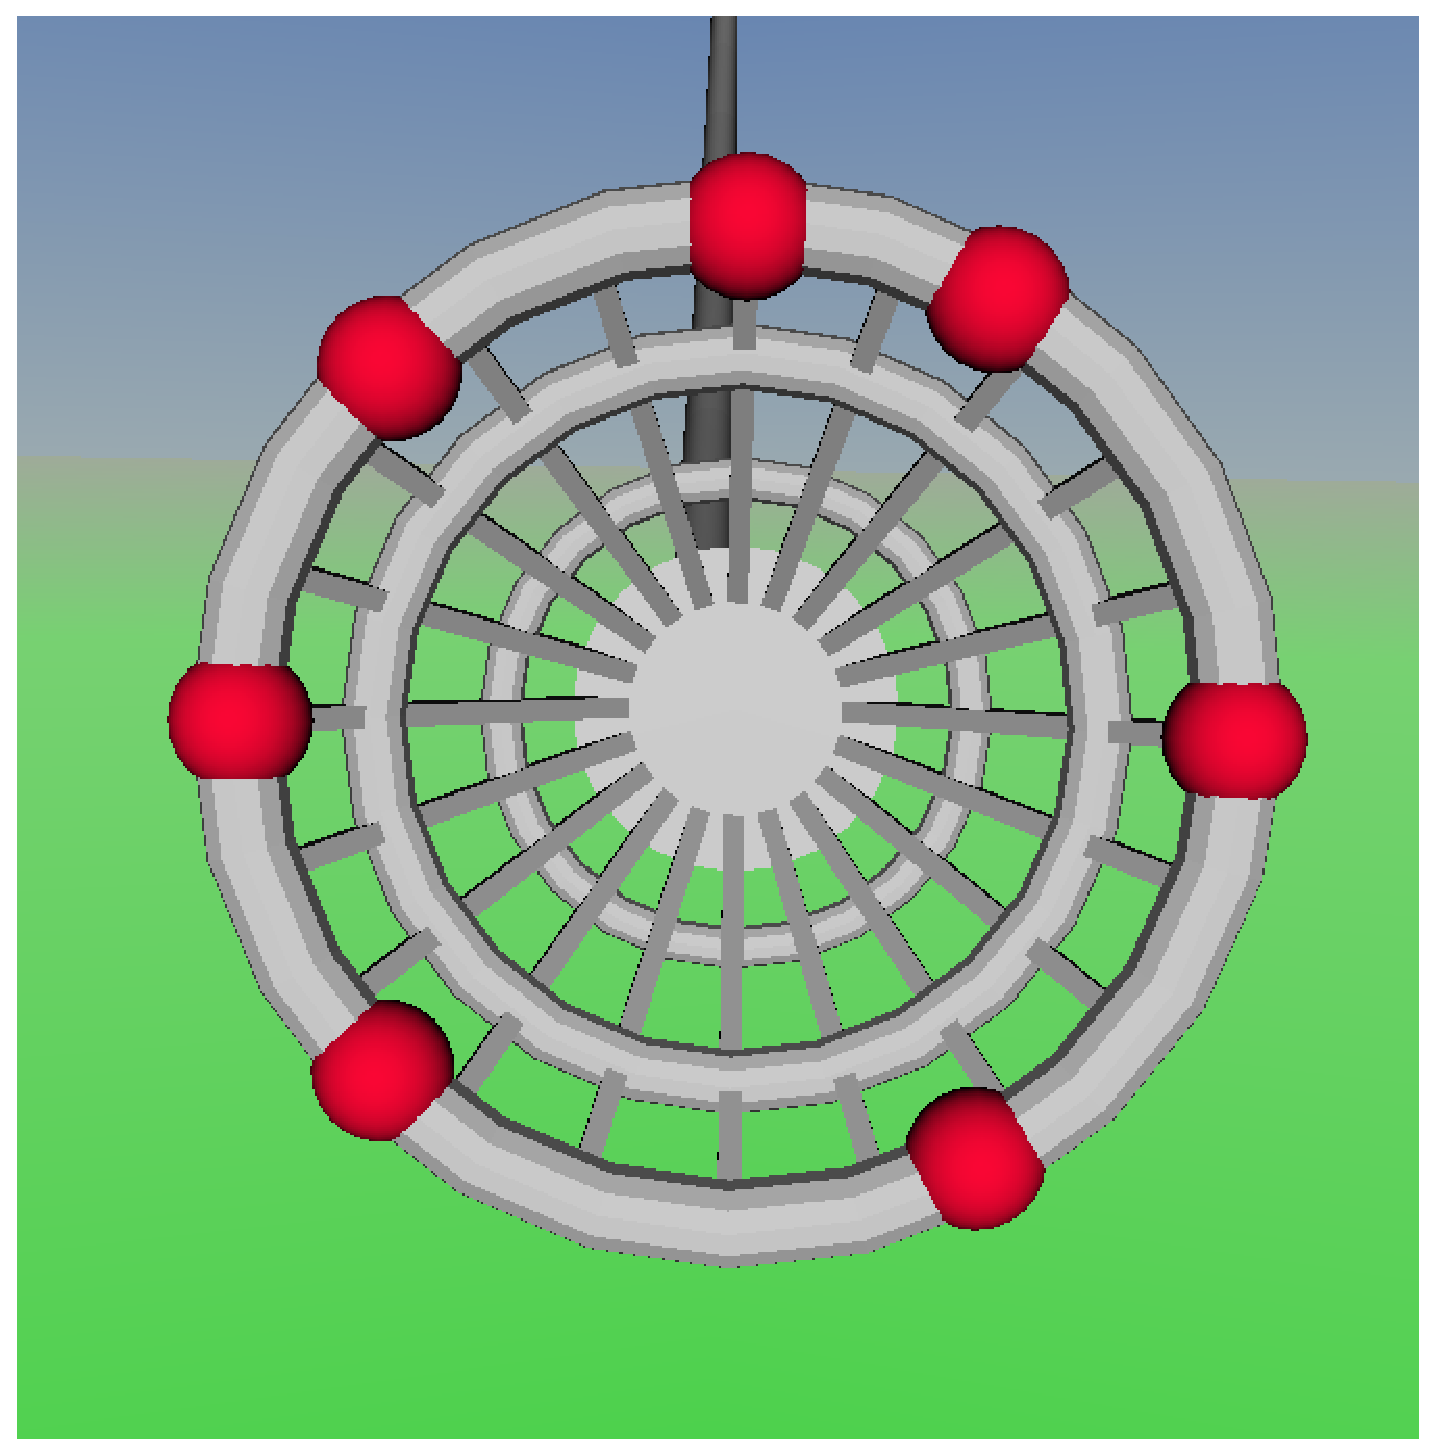
\includegraphics[width=5cm]{Figures/Figs_Ch6/drogue.eps}
	\caption{Markers located at the drogue }
	\label{fig2}
\end{figure}

\subsection{Coordinate System Transformation}

In this chapter, the coordinate systems are defined as follows (see Fig.~\ref%
{fig3}). The camera coordinate system $o_{\mathrm{c}}-x_{\mathrm{c}}y_{%
	\mathrm{c}}z_{\mathrm{c}}$ is attached to the camera. Its origin is the
optical center of the camera, with $x_{\mathrm{c}}$ axis pointing forward, $y_{%
	\mathrm{c}}$ axis pointing right, $z_{\mathrm{c}}$ axis pointing downward.
The other coordinate system is the drogue coordinate system $o_{\mathrm{d}}-x_{\mathrm{d}%
}y_{\mathrm{d}}z_{\mathrm{d}}$, whose origin is the center of the drogue. Moreover, its orientation is the same as the camera coordinate system.

Assume that vectors $\mathbf{p}_{\mathrm{c}}\triangleq \lbrack x_{\mathrm{c}%
}\ y_{\mathrm{c}}\ z_{\mathrm{c}}]^{\mathrm{T}}$ and $\mathbf{p}_{\mathrm{d}%
}\triangleq \lbrack x_{\mathrm{d}}\ y_{\mathrm{d}}\ z_{\mathrm{d}}]^{\mathrm{%
		T}}$ are in two coordinate systems above, which satisfy \cite{Zhang}: 
\begin{equation}
\mathbf{p}_{\mathrm{c}}=\mathbf{R}_{\mathrm{d}}^{\mathrm{c}}\mathbf{p}_{\mathrm{d}}+\mathbf{t}_{\mathrm{d}}^{\mathrm{c}}  \label{eq11}
\end{equation}%
where $\mathbf{R}_{\mathrm{d}}^{\mathrm{c}}\in \mathbb{R}^{3\times 3}$ is the rotation matrix, and $\mathbf{t}_{\mathrm{d}}^{\mathrm{c}}\in \mathbb{R}^{3}$ is the translation vector. 
The rotation matrix $\mathbf{R}_{\mathrm{d}}^{\mathrm{c}}$ from the drogue coordinate system to the camera coordinate system can be shown as 
\begin{equation}
\mathbf{R}_{\mathrm{d}}^{\mathrm{c}}=\mathbf{R}_{\mathrm{z}}^{\mathrm{T}}(\psi )\mathbf{R}_{\mathrm{y}}^{\mathrm{T}}(\theta )\mathbf{R}_{\mathrm{x}}^{\mathrm{T}}(\phi ).  \label{eq10}
\end{equation}
In the equation above, with three principal axes, a rotation of angle $\phi $ about the x-axis is defined as 
\begin{equation}
\mathbf{R}_{\mathrm{x}}(\phi )\triangleq 
\begin{bmatrix}
1 & 0 & 0 \\ 
0 & \cos \phi  & \sin \phi  \\ 
0 & -\sin \phi  & \cos \phi 
\end{bmatrix}.
\label{eq7}
\end{equation}
Similarly, a rotation of angle $\theta $ about the y-axis is defined as 
\begin{equation}
\mathbf{R}_{\mathrm{y}}(\theta )\triangleq 
\begin{bmatrix}
\cos \theta  & 0 & -\sin \theta  \\ 
0 & 1 & 0 \\ 
\sin \theta  & 0 & \cos \theta 
\end{bmatrix}.
\label{eq8}
\end{equation}%
Besides, a rotation of angle $\psi $ about the z-axis is defined as 
\begin{equation}
\mathbf{R}_{\mathrm{z}}(\psi )\triangleq 
\begin{bmatrix}
\cos \psi  & \sin \psi  & 0 \\ 
-\sin \psi  & \cos \psi  & 0 \\ 
0 & 0 & 1
\end{bmatrix}
\label{eq9}
\end{equation}
where $\psi $, $\theta $ and $\phi $ are the Euler angles.

In the process of aerial refueling, the rotation between the receiver
aircraft and the drogue is limited in a small range to ensure the safety,
which can be ignored. Thus, assume that there is only translation which can
be expressed as 
\begin{equation}
\mathbf{p}_{\mathrm{c}}=\mathbf{p}_{\mathrm{d}}+\mathbf{t}_{\mathrm{d}}^{\mathrm{c}}.  \label{eq36}
\end{equation}
Using~(\ref{eq36}) , equations of position parameters can be established and solved. 
\begin{figure}[!htb]
	\centering
	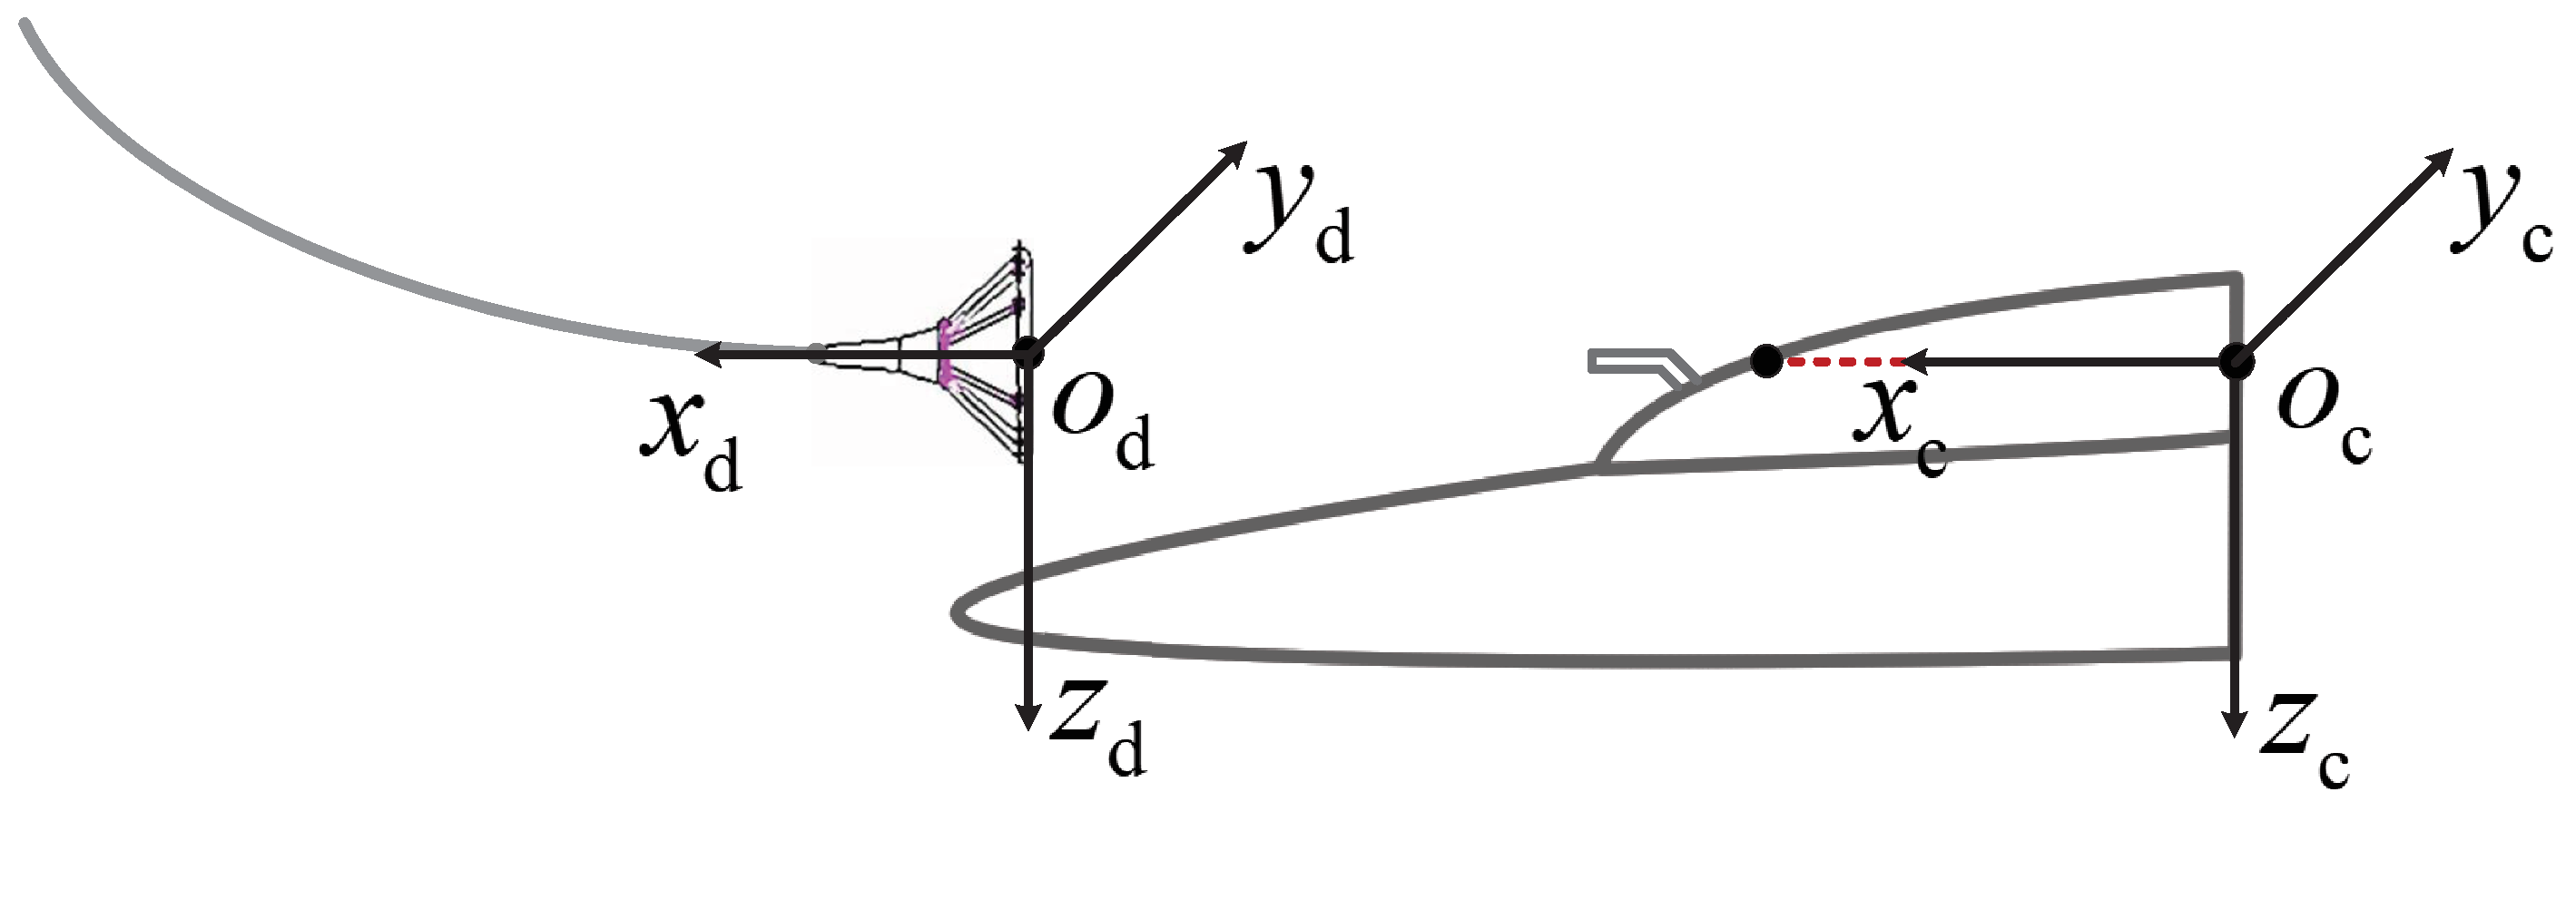
\includegraphics[width=0.6\hsize]{Figures/Figs_Ch6/refueling2.eps}
	\caption{The coordinate systems of the refueling system \cite{Zhang1}}
	\label{fig3}
\end{figure}


\subsection{Camera Pinhole Model}
Assume that a vector $\mathbf{p}_{\mathrm{i}}\triangleq \lbrack u\ v]^{\mathrm{T}}$ is in the image coordinate system $o_{\mathrm{i}}-x_{\mathrm{i}}y_{\mathrm{i}}$. The camera pinhole model (see Fig.~\ref{fig1}) is used to transform $\mathbf{p}_{\mathrm{c}}$ and $\mathbf{p}_{\mathrm{d}}$ to $\mathbf{p}_{\mathrm{i}}$ as follows 
\begin{equation}
l\!\begin{bmatrix}\! u \\ v \\ 1\!\end{bmatrix}\!\!= \!\!\begin{bmatrix}\!
\alpha _{\mathrm{x}} & 0 & u_{\mathrm{0}} & 0 \\ 0 & \alpha _{\mathrm{y}} & v_{\mathrm{0}} & 0 \\ 0 & 0 & 1 &
0\!\end{bmatrix}\!\!\begin{bmatrix}\! x_{\mathrm{c}} \\ y_{\mathrm{c}} \\ z_{\mathrm{c}} \\ 1\!\end{bmatrix}\!\\
\!=\!\mathbf{M}\!\begin{bmatrix}\! \mathbf{R}_{\rm{d}}^{\rm{c}} &
\mathbf{t}_{\rm{d}}^{\rm{c}} \\ 0 & 1\!\end{bmatrix}\!\!\begin{bmatrix}\! x_{\mathrm{d}} \\
y_{\mathrm{d}} \\ z_{\mathrm{d}} \\ 1\!\end{bmatrix}\!,   \label{eq12}
\end{equation}%
and
\begin{equation}
\mathbf{M}=
\begin{bmatrix}
\alpha _{\mathrm{x}} & 0 & u_{\mathrm{0}} \\ 
0 & \alpha _{\mathrm{y}} & v_{\mathrm{0}} \\ 
0 & 0 & 1
\end{bmatrix},
\label{eq13}
\end{equation}
where $l$ in~(\ref{eq12}) is the scaling factor; $\mathbf{M}$ is the camera intrinsic
matrix, in which $\alpha _{\mathrm{x}}$, $\alpha _{\mathrm{y}}$, $u_{\mathrm{0}}$ and $v_{\mathrm{0}}$ are
determined by camera calibration \cite{Zhang1}. 
\begin{figure}[!htb]
	\centering
	\includegraphics[width=8cm]{Figures/Figs_Ch6/cam.eps}
	\caption{Camera pinhole model \cite{Strum}}
	\label{fig1}
\end{figure}

\subsection{Problem Formulation}

According to the descriptions above, it is obtained that some markers are
placed on the drogue. Let the number of the markers be $N$. As all markers
are placed in the same plane, their depth information is identical, which
can be expressed as $s$. Thus the markers in the image can be described as $%
(u_{i},v_{i},s),\ i=1,2,\cdots,N$. Since the markers compose a circle, it
is necessary to obtain the center coordinate and radius of the circle, which
can be expressed as $(a,b,r)$ with $(a,b)$ denoting the center coordinate of the circle, $r$ the radius of
the circle. With these parameters, the relative distance
between the drogue and the receiver aircraft is obtained. However, since the external environment is complicated and full of interferences, some
essential measures should be taken, which can ensure the accuracy of the
parameters and improve the robustness of the whole system.

There are two major tasks in this chapter: drogue recognition and enhancing
detection robustness. Enhancing detection robustness is based on the prediction of
the markers' coordinates, and it can be divided into three parts corresponding to
different situations. Therefore, for simplicity, they are formulated into
the following four steps.
\begin{enumerate}[1)]
	\item Step 1: Assume that there is no disturbance and the whole refueling system works well. According to the known parameters $(u_{i},v_{i},s),\ i=1,2,\cdots,N$, get the the center and radius of the circle $(a,b,r)$.
	
	\item Step 2: According to the relative distance between the drogue and the receiver aircraft got in \textit{Step 1}, estimate the coordinates of the markers at the next moment and revise the current data.
	
	\item Step 3: Assume that there are some noise and redundant points in the image. According to the known parameters $(u_{i},v_{i},s),\ i=1,2,\cdots,N$ and the equation of the circle, eliminate the influence of interferences.
	
	\item Step 4: Assume that there are some markers undetectable. According to the current and predictive coordinates of the markers, bring forward corresponding measures.
\end{enumerate}

Next, the main algorithm will be introduced in Section \uppercase\expandafter{\romannumeral3} in detail.

\section{Main Algorithm for Position Estimation}
\subsection{Markers Detecting and Matching}
As shown above, markers placed on the drogue are arranged as a circle. In
the process of aerial refueling, the receiver aircraft should track the
tanker aircraft with high accuracy. Thus, the angle of attack of the receiver
aircraft is very small, according to which the drogue can be approximated as
a circle. Its projection on the image can be expressed in the function form
as 
\begin{equation}
\left( x-a\right) ^{2}+(y-b)^{2}=r^{2}  \label{eq1}
\end{equation}
Let $N$ be the number of all detected markers. The detected markers can be expressed as
$\mathbf{p}_{i}\triangleq[x_{i}\ y_{i}]^{\mathrm{T}},\ i=1,2,\cdots,N$.
In order to describe the difference between the observed value and the
estimated value, the residuals $\varepsilon _{i}$ is used, which can be shown
as 
\begin{equation}
\varepsilon _{i}=\left( x_{i}-a\right) ^{2}+(y_{i}-b)^{2}-r^{2}.  \label{eq2}
\end{equation}
The cost function can be the sum of the residuals' square, that is 
\begin{equation}
J=\sum_{i=1}^{N}\varepsilon _{i}^{2}=\sum_{i=1}^{N}\left[ \left(x_{i}-a\right) ^{2}+(y_{i}-b)^{2}-r^{2}\right]^{2}.  \label{eq3}
\end{equation}

According to the principle of the least square, when the partial derivative of the
cost function equals zero, the optimal fitting result is achieved, which can be written in the numerical form as 
\begin{equation}
\!\left\{ \! \!
\begin{array}{l}
\! \cfrac{\partial J}{\partial a}\!=\!-4(x_{i}\!-\!a)\sum\limits_{i=1}^{N}%
\left[ \left( x_{i}\!-\!a\right) ^{2}\!+\!(y_{i}\!-\!b)^{2}\!-\!r^{2}\right]%
\!=\!0 \\ 
\cfrac{\partial J}{\partial b}\!=\!-4(y_{i}\!-\!b)\sum\limits_{i=1}^{N}%
\left[ \left( x_{i}\!-\!a\right) ^{2}\!+\!(y_{i}\!-\!b)^{2}\!-\!r^{2}\right]%
\!=\!0 \\ 
\cfrac{\partial J}{\partial r}\!=\!-4r\sum\limits_{i=1}^{N}\left[ \left(
x_{i}\!-\!a\right) ^{2}\!+\!(y_{i}\!-\!b)^{2}\!-\!r^{2}\right]\!=\!0 .
\end{array}
\right.  \label{eq4}
\end{equation}
With these functions, the parameters of the circle are obtained as 
\begin{equation}
\left\{ 
\begin{array}{l}
\begin{aligned} a=\ &\cfrac{(\overline{x^{2}}\cdot
	\overline{x}+\overline{x}\cdot
	\overline{y^{2}}-\overline{x^{3}}-\overline{xy^{2}})(\overline{y}^{2}-
	\overline{y^{2}})}{2(\overline{x}^{2}-\overline{x^{2}})(\overline{y}^{2}-
	\overline{y^{2}})-2(\overline{x}\cdot \overline{y}-\overline{xy})^{2}}\ -\\
&\cfrac{(\overline{x^{2}}\cdot \overline{y}+\overline{y}\cdot
	\overline{y^{2}}-\overline{x^{2}y}-\overline{y^{3}})(\overline{x}\cdot
	\overline{y}-\overline{xy})}{2(\overline{x}^{2}-\overline{x^{2}})(
	\overline{y}^{2}-\overline{y^{2}})-2(\overline{x}\cdot
	\overline{y}-\overline{xy})^{2}}\end{aligned}\vspace{2ex} \\ 
\begin{aligned} b=\ &\cfrac{(\overline{x^{2}}\cdot
	\overline{y}+\overline{y}\cdot
	\overline{y^{2}}-\overline{x^{2}y}-\overline{y^{3}})(\overline{x}^{2}-
	\overline{x^{2}})}{2(\overline{x}^{2}-\overline{x^{2}})(\overline{y}^{2}-
	\overline{y^{2}})-2(\overline{x}\cdot \overline{y}-\overline{xy})^{2}}\ -\\
&\cfrac{(\overline{x^{2}}\cdot \overline{x}+\overline{x}\cdot
	\overline{y^{2}}-\overline{x^{3}}-\overline{xy^{2}})(\overline{x}\cdot
	\overline{y}-\overline{xy})}{2(\overline{x}^{2}-\overline{x^{2}})(
	\overline{y}^{2}-\overline{y^{2}})-2(\overline{x}\cdot
	\overline{y}-\overline{xy})^{2}}\end{aligned}\vspace{2ex} \\ 
r=\sqrt{a^{2}-2\overline{x}a+b^{2}-2\overline{y}b+\overline{x^{2}}+\overline{
		y^{2}}}\vspace{2ex}
\end{array}
\right.  \label{eq5}
\end{equation}
where $\overline{x}$ and $\overline{y}$ denote the average values of $x$ and $y$, and $\overline{x^{m}y^{n}}=\cfrac{\sum_{i=1}^{N}x_{i}^{m}y_{i}^{n}}{N}, m, n\in[0,3]$.

On the basis of camera pinhole model, the depth $s$ of the plane at which
the markers are located can be obtained by the radius of the circle. The
function is as follows
\begin{equation}
\frac{R_{\mathrm{dr}}}{s+f}=\frac{r}{f}  \label{eq14}
\end{equation}%
where $R_{\mathrm{dr}}$ is the actual radius, $f$ is the focal length of the camera.
Let the coordinate of the probe in the image be $\mathbf{p}_{\mathrm{i}}\triangleq
\lbrack u\ v]^{\mathrm{T}}$, and the distance between the probe and the camera in z-axis be $d$. The relative distance
between the drogue and the probe can be expressed as 
\begin{equation}
\left\{ 
\begin{array}{l}
\Delta x=\left\vert a-u\right\vert \cdot \cfrac{R_{\mathrm{dr}}}{r}\vspace{1ex} \\ 
\Delta y=\left\vert b-v\right\vert \cdot \cfrac{R_{\mathrm{dr}}}{r}\vspace{1ex} \\ 
\Delta z=\left\vert \dfrac{fR_{\mathrm{dr}}}{r}-f-d\right\vert \vspace{1ex}.
\end{array}
\right.
\end{equation}

Although the form of this algorithm is complex, its time complexity is just $%
O(n)$, which is suitable for computer implementation.

\subsection{KF and Robust Image Tracking Algorithm}

In this subsection, KF is applied to estimate the position of
markers, which can reduce the influence of error points and improve the
matching accuracy. The equations of state and measurement are
given as follows 
\begin{equation}
\mathbf{x}(k+1)\!=\!\mathbf{\Phi }(k+1,k)\mathbf{x}(k)\!+\!\ \mathbf{\Gamma }%
(k+1,k)\mathbf{W}(k)  \label{eq15}
\end{equation}%
\begin{equation}
\mathbf{z}(k)=\mathbf{H}(k)\mathbf{x}(k)+\mathbf{V}(k).  \label{eq16}
\end{equation}
In above functions, $\mathbf{x}(k)\in \mathbb{R}^{6}$ is the state vector of
the system state, which is written as 
\begin{equation}
\mathbf{x}=
\begin{bmatrix}
\Delta x & \Delta y & \Delta z & \Delta v_{\mathrm{x}} & \Delta v_{\mathrm{y}} & \Delta v_{\mathrm{z}}%
\end{bmatrix}
^{\mathrm{T}}  \label{eq17}
\end{equation}
where $\Delta x,\Delta y,\Delta z$ are the relative distances between the
receiver aircraft and the drogue along three axes, respectively. And $\Delta v_{\mathrm{x}},\Delta v_{\mathrm{y}},\Delta
v_{\mathrm{z}} $ are velocity differences; $\mathbf{z}(k)\in \mathbb{R}^{3}$ is the observation vector, which is expressed as 
\begin{equation}
\mathbf{z}=
\begin{bmatrix}
u & v & s
\end{bmatrix}
^{\mathrm{T}}.  \label{eq23}
\end{equation}
and $\mathbf{H}(k)$ can be obtained from the correspondence of the image and the real world.
Besides, other parameters can be expressed as 
\begin{equation}
\mathbf{\Phi }(k+1,k)=
\begin{bmatrix}
\mathbf{0}_{3} & \mathbf{I}_{3} \\ 
\mathbf{0}_{3} & \mathbf{0}_{3}
\end{bmatrix}
\label{eq18}
\end{equation}
\begin{equation}
\mathbf{\Gamma }(k+1,k)=
\begin{bmatrix}
\mathbf{0}_{3} \\ 
\mathbf{I}_{3}
\end{bmatrix}.
\label{eq20}
\end{equation}

Given the initial value, the well-known KF consisting of prediction and estimation parts can start to
iterate. The estimation of the states can be sent to the autopilot for the docking control. KF can also improve the
system robustness performance enormously which will ensure the normal
operation of the whole refueling system.

\subsection{The Dispose of Noise and Redundant Points}

As the environment around the refueling equipment is complex, it is a common
phenomenon that some noise and redundant points appear in the image, which may affect the matching of the drogue. These redundant points may
emerge for the following reasons: direct sunlight, light reflecting on
the surface of the tanker aircraft, the noise points generated by the
camera. The corresponding measures are given as follows.

For the drogue of the refueling system, let the center coordinate of
estimation in world space be $\mathbf{z}=[\Delta x\ \Delta y\ \Delta z]{}^{%
	\mathrm{T}}$. According to the projection relation, the next center and
radius of the circle in the image can be forecasted as $(a,b)$ and $r$, and
the estimation errors are $\Delta a$, $\Delta b$, $\Delta r$, respectively.
For the image point $(u,v)$ at the next moment, the judgment rules can be
expressed as follows 
\begin{equation}
\sqrt{(u_{i}-a)^{2}+\left( v_{i}-b\right) ^{2}}>\sqrt{\Delta a^{2}+\Delta
	b^{2}}+r+\Delta r  \label{eq33}
\end{equation}
or 
\begin{equation}
\sqrt{(u_{i}-a)^{2}+\left( v_{i}-b\right) ^{2}}<r-\Delta r.  \label{eq34}
\end{equation}
The two formulas have a similar effect, which can distinguish the unwanted
points with high efficiency. If the point satisfies the condition (\ref{eq33}) or (\ref{eq34}), it will
be removed.

In addition, as the markers located at the drogue are placed as a circle,
let the current circle in the image be $(a,b,r)$. If the fitting error
is greater than the threshold value $\varepsilon $ set earlier, this point should be
removed. The function can be expressed as 
\begin{equation}
\frac{(u_{i}-a)^{2}+(v_{i}-b)^{2}-r^{2}}{r}>\varepsilon.  \label{eq35}
\end{equation}
In actual operation, the value of $\varepsilon $ can be got from real
experiments.

The first algorithm shown above removes the unsuitable points in the aspect
of the markers' movement tendency, while the other does the same in the aspect of markers'
geometry distribution property. Together with other necessary logical
judgments, most errors can be discovered and got rid of, which can
ensure the accuracy of position estimation.

\subsection{The Algorithm of Losing Points}

When the probe-and-drogue refueling system is operating, there is a common
phenomenon that some of the markers may be out of the camera's view or
obscured by the probe or other obstacles. Due to the determination of
parameters of the circle $(a,b,r)$, three detectable markers should
be obtained at least. By estimating the coordinates of the markers in the image,
whether or not there are markers out of sight can be determined in advance.
Different states and necessary countermeasures are listed as follows.

State 1: If some of the markers are out of sight, and other visible markers
are near the probe, this situation means that the invisible markers are obscured by the
probe. If they are just out of sight for a short time, which is less than the
threshold value $t_{\mathrm{i}}$ , the estimation results of KF can fill
the missing data directly, which can maintain system normal operation. However, at the same
time, an alarm is provided until all return to normal.

State 2: If some markers are blocked by the probe for such a long time that
exceeds the threshold value $t_{\mathrm{i}}$ , it is necessary to check the number of
markers available. If the number is less than three, it is illustrated that
the position estimation system is in bad condition, which may lead to huge
safety risks. Thus, the receiver aircraft should stop refueling process
immediately. Until the receiver aircraft returns to a safe place, a next
refueling attempt is allowed to begin.

State 3: If some markers are out of sight, and the existing markers
are near the four boundaries of the camera's view, it means that the
invisible markers are beyond the camera's view. If this situation occurs,
it implies that there is something wrong with the relative position between
the receiver aircraft and the tanker aircraft. If all the missing markers
return to view after a short period, which is less than the threshold value $t_{\mathrm{p}}$, the refueling process can be permitted to carry on. If not, the refueling process must be stopped at once. An alarm is
also required in this situation.

The threshold values $t_{\mathrm{i}}$ and $t_{\mathrm{p}}$ can be got from real experiments.
However, according to the intensity of the events, $t_{\mathrm{p}}$ is much smaller than $%
t_{\mathrm{i}} $. With these countermeasures, the robustness of the whole refueling
system can be highly improved.

\section{Deep Learning-Based Drogue Detection}

The target-based detection algorithms are susceptible to light interference and sensitive to weather conditions. Object detection algorithms based on deep learning, on the other hand, can directly learn the features of objects from images, eliminating the need for target installation on drogue and providing strong robustness. Early object detection algorithms consisted of two steps, namely candidate box generation and candidate box classification and localization, referred to as two-stage algorithms, such as R-CNN\cite{girshick2014rich}, Faster-RCNN\cite{ren2015faster}, and FPN\cite{lin2017feature}. In contrast to two-stage algorithms, one-stage algorithms merge the two steps into one, significantly improving detection speed. Examples of one-stage algorithms include YOLO\cite{redmon2016you}, SSD\cite{fu2017dssd}, and RetinaNet\cite{lin2017focal}, with the YOLO series being the most widely used at present. In this chapter, the YOLOv5 algorithm is employed for drogue detection.

\subsection{Network Architecture}

The network architecture of YOLOv5 is illustrated in Fig.~\ref{YOLO-network} and can be divided into four components: Input, Backbone, Neck, and Output. A key feature of YOLOv5 is its ability to detect objects on three different scales of feature maps, obtained through downsampling, corresponding to 1/32, 1/16, and 1/8 of the input image dimensions. The largest feature map is responsible for detecting small objects. For each point on the feature map, predictions are made using three anchor boxes as priors.

\begin{figure}[!htb]
	\centering
	\includegraphics[width=11cm]{Figures/Figs_Ch6/YOLO-network.eps}
	\caption{The network architecture of YOLOv5}
	\label{YOLO-network}
\end{figure}

\subsubsection{Input}

(i) \textbf{Mosaic data augmentation}. The Mosaic data augmentation method was introduced in YOLOv4\cite{bochkovskiy2020yolov4}. Its main idea is to concatenate four images together by randomly scaling, cropping, and arranging them. This concatenated image is then used as training data. The advantage of this approach is that it enhances the background diversity of the images and effectively increases the training batch size by combining four images into one.

(ii) \textbf{Adaptive anchor box computation}. In the algorithm, initial anchor boxes with predefined aspect ratios are set for different datasets. During the training process, the network computes predicted boxes based on these initial anchor boxes, compares them with the ground truth boxes, measures the differences between the two, and then updates the network parameters in a backward manner. YOLOv5 incorporates the functionality of adaptive computation of initial anchor boxes into the code, automatically calculating the optimal anchor box values for different training sets during each training iteration.

(iii) \textbf{Adaptive image scaling}. In the process of collecting datasets, it is common for images to have varying dimensions. A commonly used approach is to uniformly scale the images during data preprocessing to obtain a standardized size before inputting them into the network. Popular sizes used in the YOLO algorithm include $416 \times 416$ and $608 \times 608$. To achieve the standardized size, padding is applied to the edges of the images that fall short after scaling. In the prediction stage, YOLOv5 optimizes the padding algorithm, minimizing the extent of padding required and thereby improving the speed of object detection.

\subsubsection{Backbone}

(i) \textbf{Focus structure}. The most critical aspect of the Focus structure is the slicing operation. In YOLOv5, a $608 \times 608 \times 3$ image enters the Focus structure, undergoes the slicing operation, resulting in a $304 \times 304 \times 12$ feature map. Subsequently, a convolution operation with a kernel size of 32 is performed, transforming it into a $304 \times 304 \times 32$ feature map.

(ii) \textbf{CSP structure}. The CSP structure, inspired by CSPNet\cite{wang2020cspnet}, addresses the issue of excessive computational complexity in inference from the perspective of network architecture design. YOLOv5 incorporates two types of CSP structures, with the CSP1\_X structure applied to the Backbone and the CSP2\_X structure utilized in the Neck.

\subsubsection{Neck}
The Neck network employs the FPN+PAN structure, drawing inspiration from PANet\cite{liu2018path}. FPN is a top-down structure that utilizes upsampling to propagate and fuse high-level feature information, generating feature maps for prediction. YOLOv5 introduces a bottom-up feature pyramid after the FPN layer, which includes two RAN structures. By combining these two components, the FPN structure can transmit strong semantic features from top to bottom, while the feature pyramid is responsible for propagating strong localization features from bottom to top. The combination of these two components performs parameter aggregation operations on different detection layers from different backbone layers.

\subsubsection{Output}

(i) \textbf{Loss function}. The loss function for object detection tasks typically consists of two components: classification loss and bounding box regression loss. YOLOv5 adopts the CIoU Loss\cite{zheng2021enhancing} as its loss function, which is derived from the DIoU Loss\cite{zheng2020distance}. The CIoU Loss combines the considerations of overlapping area, center point distance, and aspect ratio of bounding boxes. It can be represented as

\begin{equation}
L_\text{CIoU} = 1 - \text{CIoU} = 1 - (\text{IoU } - \frac{\text{Distance\_2} ^ 2 }{\text{Distance\_C} ^ 2 } - \frac{v^2}{(1-\text{IoU})+v}   )
\label{eq_loss}
\end{equation}
where $v$ is defined as a measure of aspect ratio consistency, plays a role in assessing the consistency of object's width and height ratios. It is defined as
\begin{equation}
v=\frac{4}{\pi ^2}(\arctan \frac{w^{gt}}{h^{gt}}-\arctan \frac{w^{p}}{h^{p}}).
\label{eq_v}
\end{equation}

(ii) \textbf{Non-Maximum suppression}. During the post-processing stage of object detection, multiple bounding boxes may be predicted for a single object, leading to overlapping detections. Non-Maximum Suppression (NMS) is commonly employed to identify the most relevant bounding box among them. Since CIoU incorporates the factor v, and there is no ground truth information available during prediction, DIoU is used instead. Firstly, the boxes for a specific class are sorted in descending order based on their confidence scores. Next, DIoU is computed, and boxes with DIoU values below a threshold are retained. Finally, the resulting output consists of the object's center position $(u,v )$, width $w$, height $h$, confidence score $p$, and class probability $c_0,c_1,c_2,\dots,c_{nc-1}$, as depicted in Fig.~\ref{YOLO-output}.

\begin{figure}[!htb]
	\centering
	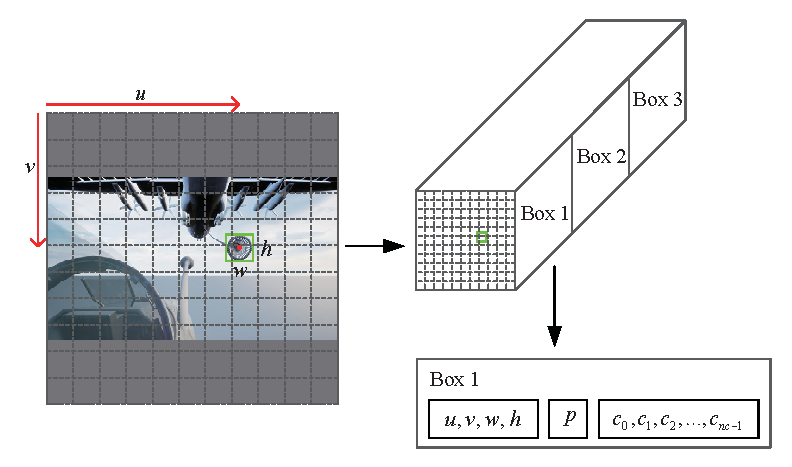
\includegraphics[width=13cm]{Figures/Figs_Ch6/YOLO-output.eps}
	\caption{The network architecture of YOLOv5}
	\label{YOLO-output}
\end{figure}

Among them, $nc$ represents the number of categories, and the class probabilities are represented as a vector of length $nc$. The index corresponding to the maximum value in the vector indicates the predicted class. Since only the detection of a single object, namely "drogue" is performed, $nc$ is set to 1.

\subsection{Position esitimation}
From the depth image, the depth value $s$ of the drogue's center point coordinates $(u, v)$ can be obtained. Using~(\ref{eq12}), the cone cover's coordinates $p_c$ in the camera coordinate system can be derived, which subsequently leads to the calculation of $p_d$.

\subsection{Dataset}
In AARSim, the data collection process for the dataset is highly convenient. By adjusting the position of the tanker, images can be obtained at arbitrary distances and angles. Additionally, the camera resolution can be adjusted, with a resolution of $1280 \times 720$ set for this experiment.

\subsection{Training approach}
The experiment was conducted using an Intel(R) Core(TM) i7-10700F CPU, 32GB of RAM, and an NVIDIA RTX 2060 SUPER 8G GPU, on the Windows 11 operating system. PyCharm was utilized for development, and training, validation, and testing were performed with the same parameters. The training parameter settings for the experiment are presented in Table \ref{tab_parameter}.

\begin{table}
	\caption{The training parameter settings for the experiment}
	
	\begin{centering}
		\begin{tabular}{|c|c|}
			\hline 
			Parameters & Value\tabularnewline
			\hline 
			Model & YOLOv5s\tabularnewline
			\hline 
			Epochs & 300\tabularnewline
			\hline 
			Image size & $640 \times 640$\tabularnewline
			\hline 
			Batch size & 16\tabularnewline
			\hline 
			Learning rate & 0.01\tabularnewline
			\hline 
			Optimizer & SGD\tabularnewline
			\hline 
		\end{tabular}
		\par\end{centering}
	\centering{}\label{tab_parameter}
\end{table}

\section{Simulation and Results}
\subsection{Simulation Environment}

In order to observe the simulation results intuitively, a three-dimensional (3D) simulation model is
created by the virtual reality toolbox of Matlab, which emulates the process of
aerial refueling precisely. The interface of this model is shown as follows
(see Fig.~\ref{fig4}). 
\begin{figure}[!htb]
	\centering
	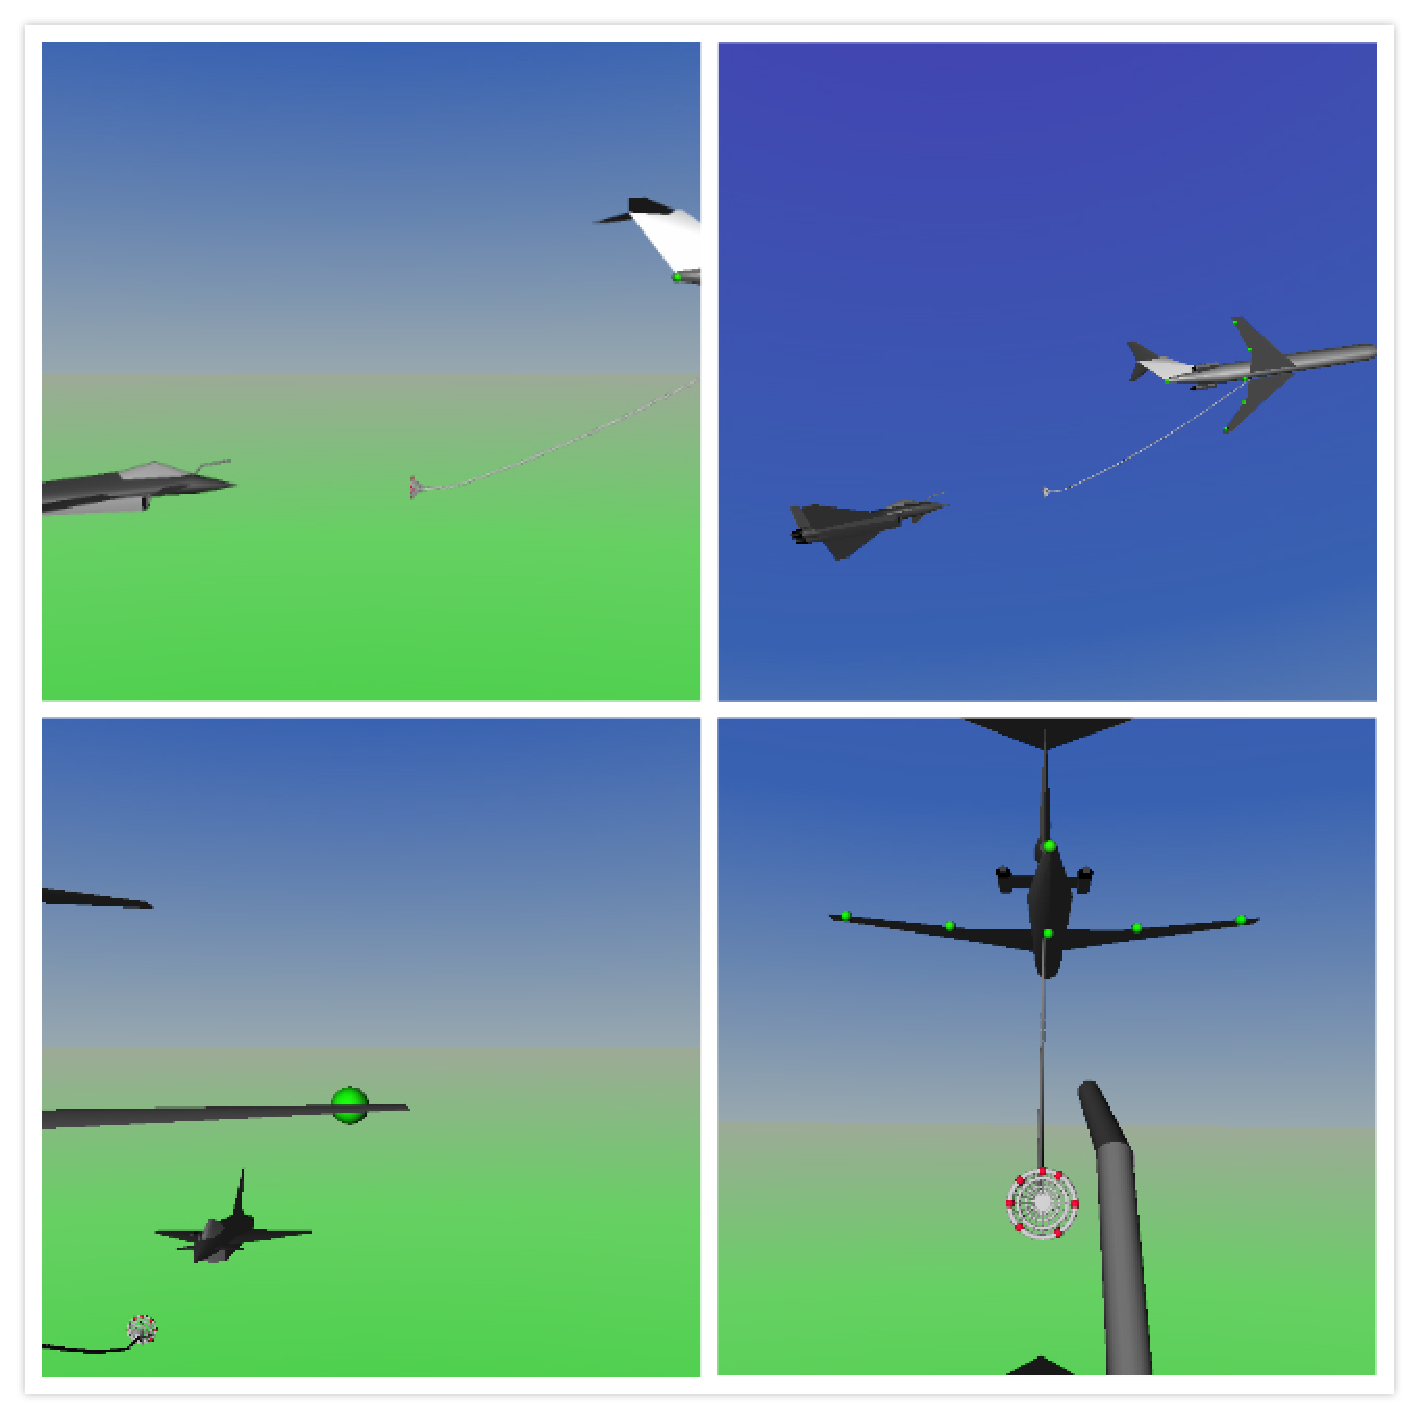
\includegraphics[width=10cm]{Figures/Figs_Ch6/jiemianhecheng.eps}
	\caption{Aerial refueling of VR simulation. }
	\label{fig4}
\end{figure}

The coordinate system of the virtual camera in this simulation model is
different from the one in Section 2. Its origin is the current location set
by the user, with $x_{\rm{c}}$ axis pointing forward, $y_{\rm{c}}$ pointing upward, $%
z_{\rm{c}}$ pointing right. In addition, the pixel resolution of the virtual
camera is 860 pixels $\times$ 480 pixels. Moreover, its maximum frame rate is 50 frames
per second. What is more, its angle of view is 90 degrees.

In order to test the effectiveness and practicability of the vision-based
algorithm proposed in Section \uppercase\expandafter{\romannumeral3}, let the drogue stay still in a series of
simulations, and at the same time, the receiver aircraft moves along the
trajectory set in advance, for example, sinusoidal movement in three axes.
According to the image acquired by the virtual camera on the receiver aircraft, the
relative distance between the receiver aircraft and the drogue can be calculated.

\subsection{Marker Identification}

For the convenience of establishing the model, some colored spheres
substitute for the passive reflectors are attached to the drogue and the
tanker aircraft. The color of the spheres on the drogue is set to be red,
while green on the tanker aircraft. The two kinds of spheres are distinguished
by color, and then treated differently.

In the image obtained by the virtual camera, the markers appear to be
bright. Thus, image gray processing~(\ref{eq37}) and thresholding function~(%
\ref{eq38}) are sufficient to detect markers. Then erode the bright pixel
blob to eliminate noise according to the threshold value $w$. Finally, the center coordinates of the pixel blob
can be obtained, namely, pixel coordinates of the markers. 
\begin{equation}
\mathbf{Gray}(u,v)=2\mathbf{R}(u,v)-\mathbf{G}(u,v)-\mathbf{B}(u,v)  \label{eq37}
\end{equation}
\begin{equation}
\mathbf{Gray}(u,v)=\left\{ 
\begin{array}{l}
255,\ if\ \mathbf{Gray}(u,v)\geq w \\ 
0,\ otherwise
\end{array}
\right.  .\label{eq38}
\end{equation}

\subsection{Simulation Results}

The whole simulation lasts for 200 seconds, while real-time pictures are
displayed in two windows. The images of different situations are listed as
follows (see Figs.~\ref{fig5} and \ref{fig6})

\begin{figure}[!htb]
	\centering
	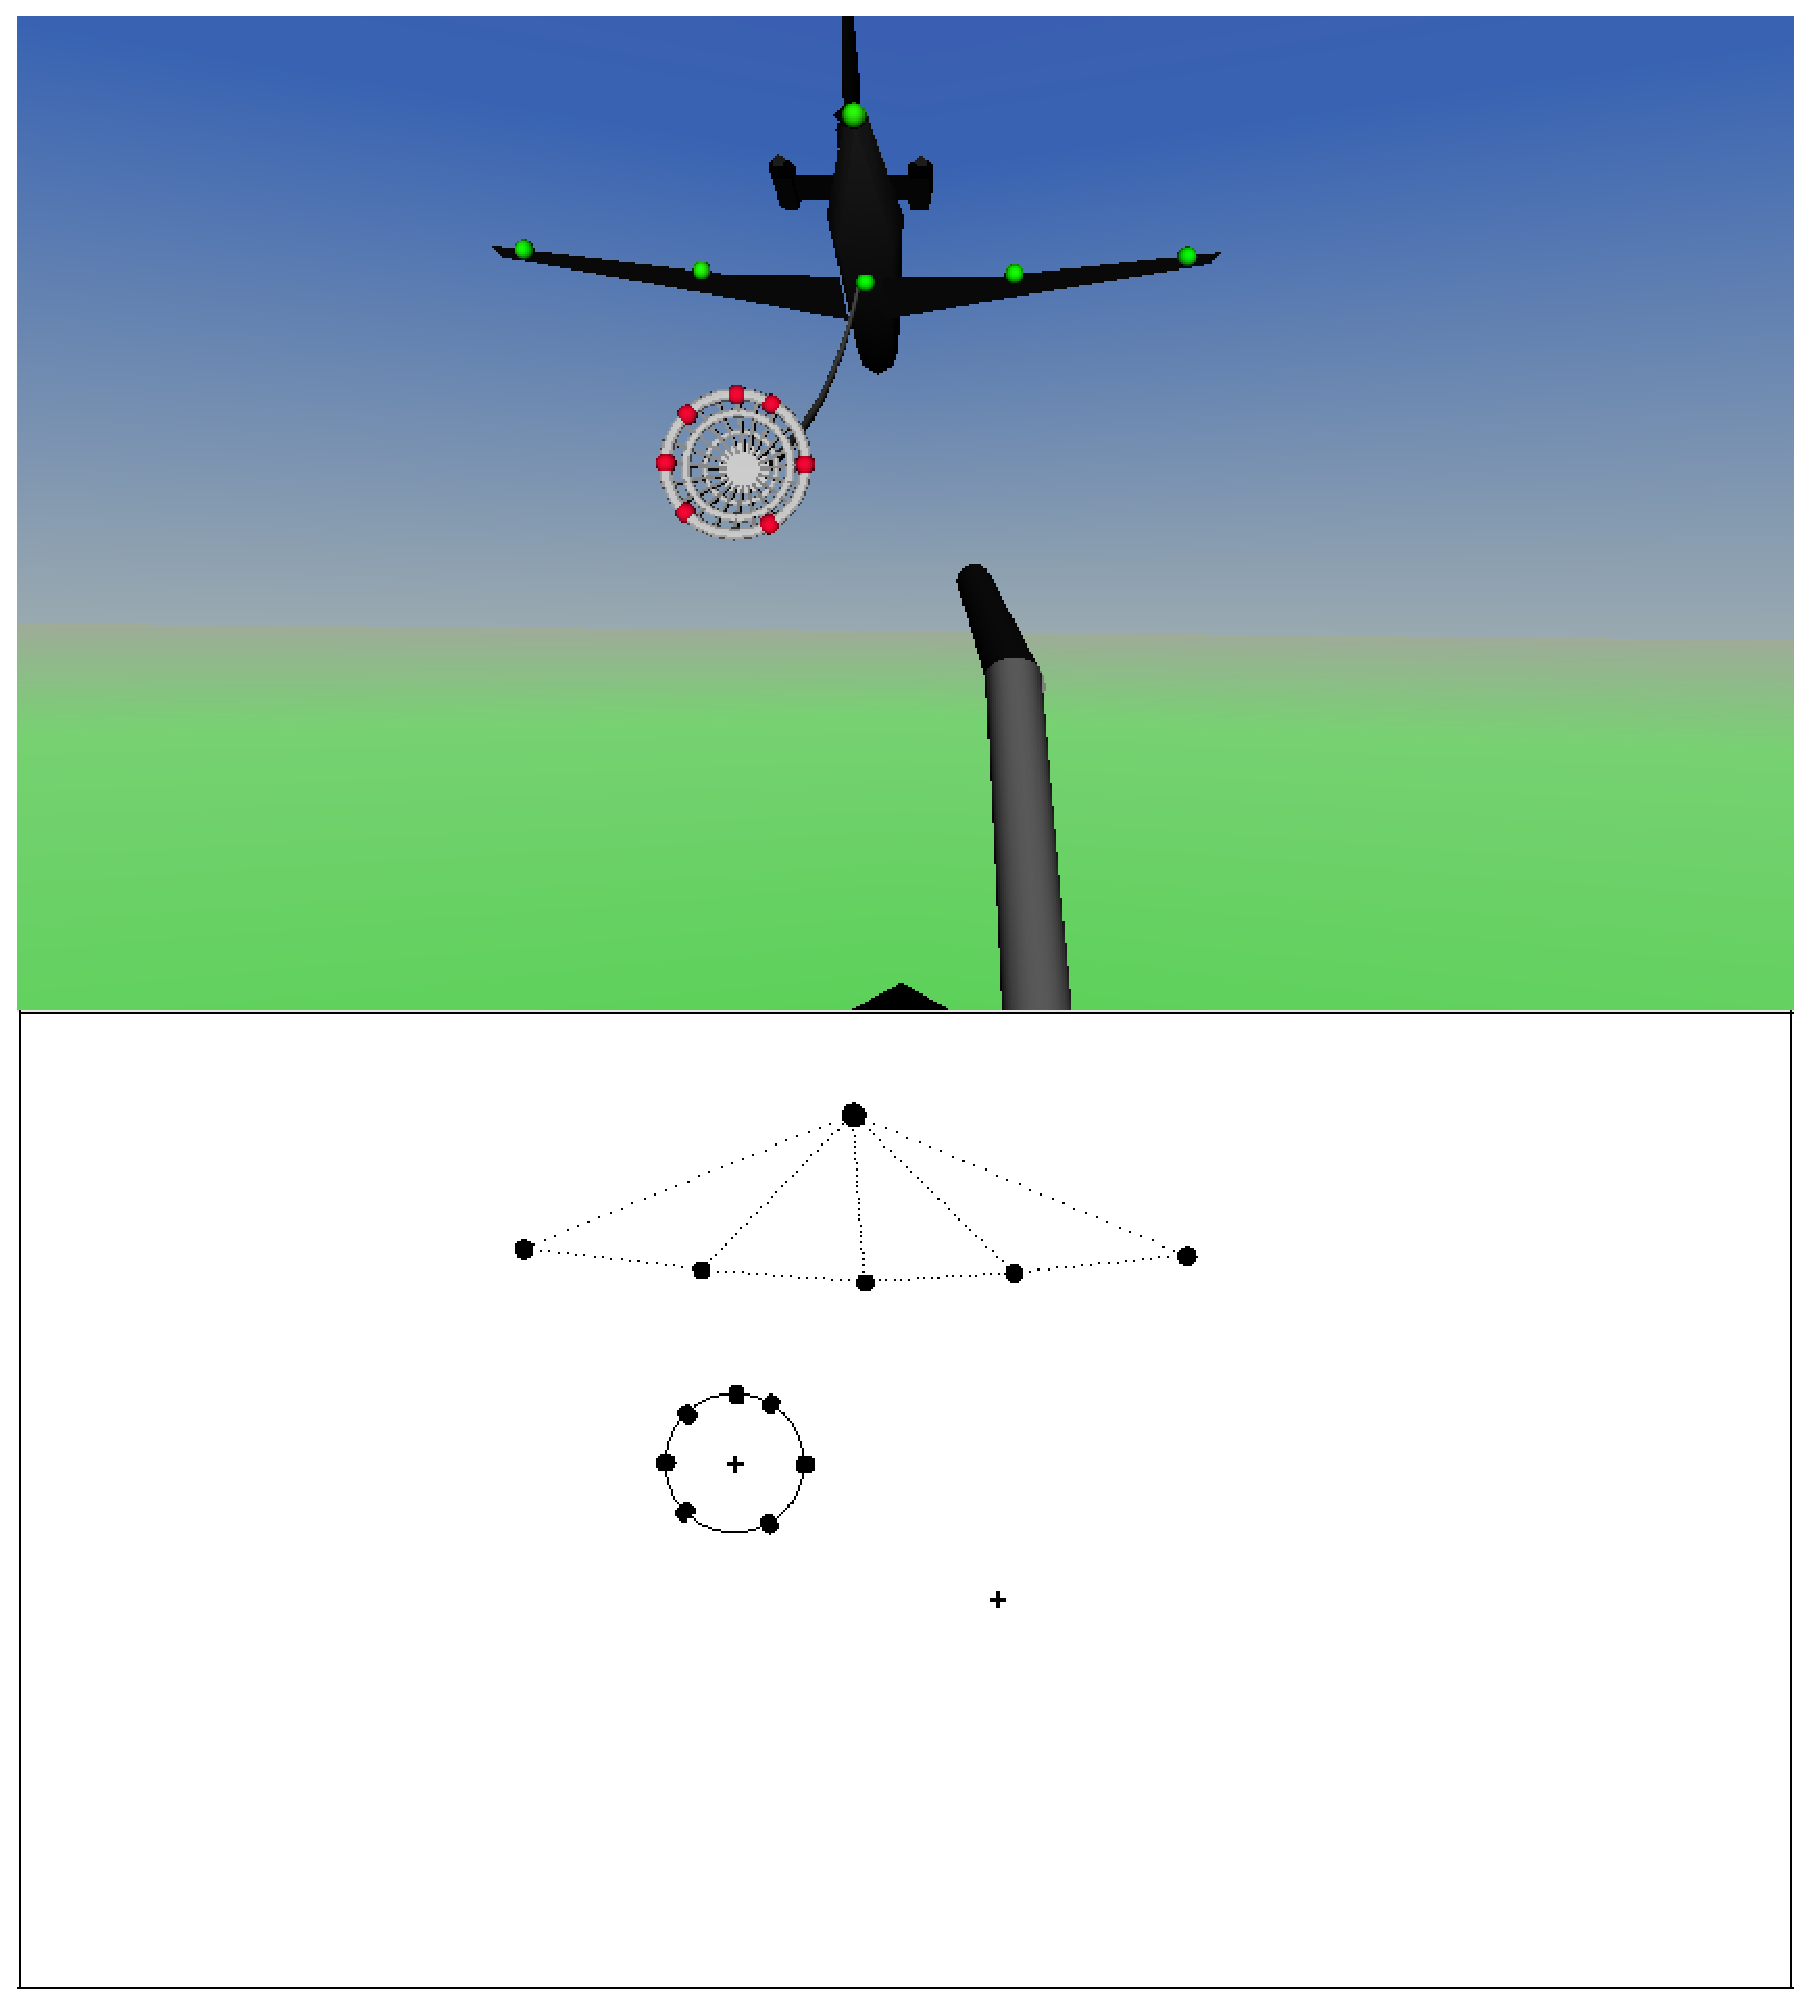
\includegraphics[width=9cm]{Figures/Figs_Ch6/fangzhen1.eps}
	\caption{All markers are identified properly}
	\label{fig5}
\end{figure}

\begin{figure}[!htb]
	\centering
	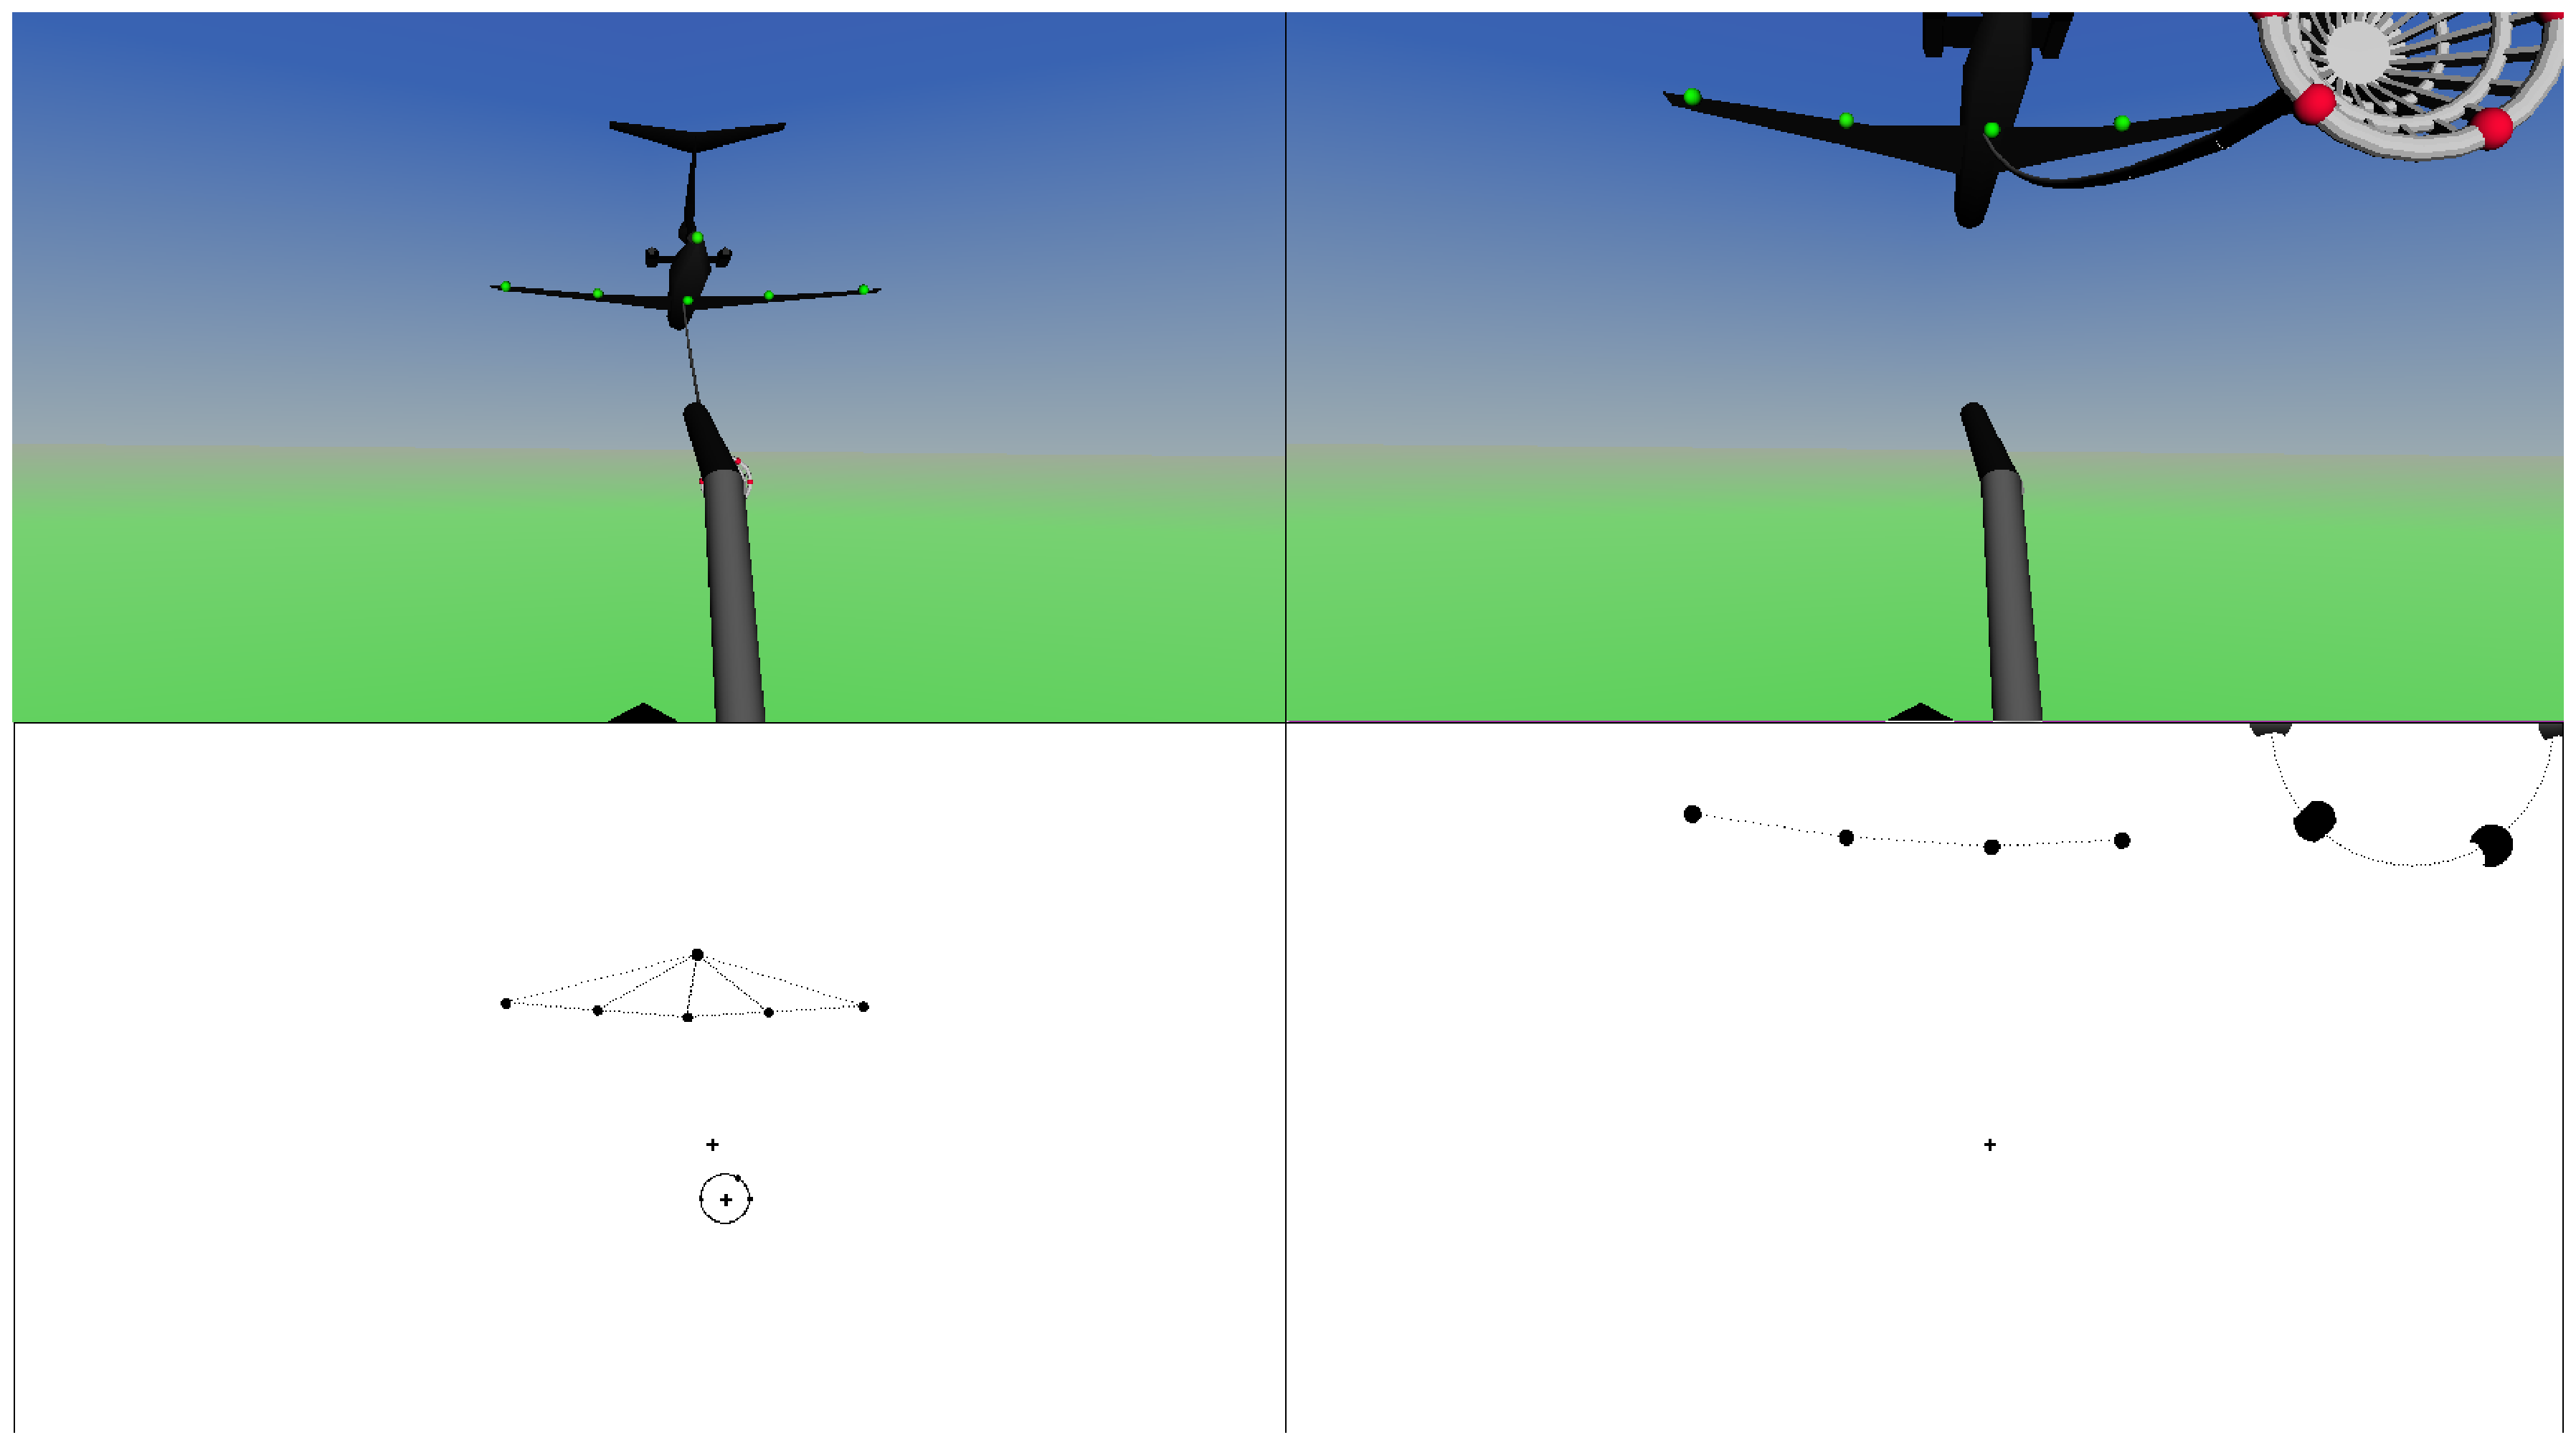
\includegraphics[width=0.7\hsize]{Figures/Figs_Ch6/fangzhen23.eps}
	\caption{85\% and 50\% of the drogue is blocked.}
	\label{fig6}
\end{figure}

From these figures, it is obtained that the circle matching algorithm can
work well even if some markers are blocked or beyond the boundary. Besides, even
though the external environment is complex, the system can ensure a
high-precision position estimation. These results show the high
robustness of this position estimation system. The positioning data and
actual data are compared as follows (see Fig.~\ref{fig8}) 
\begin{figure}[!htb]
	\centering
	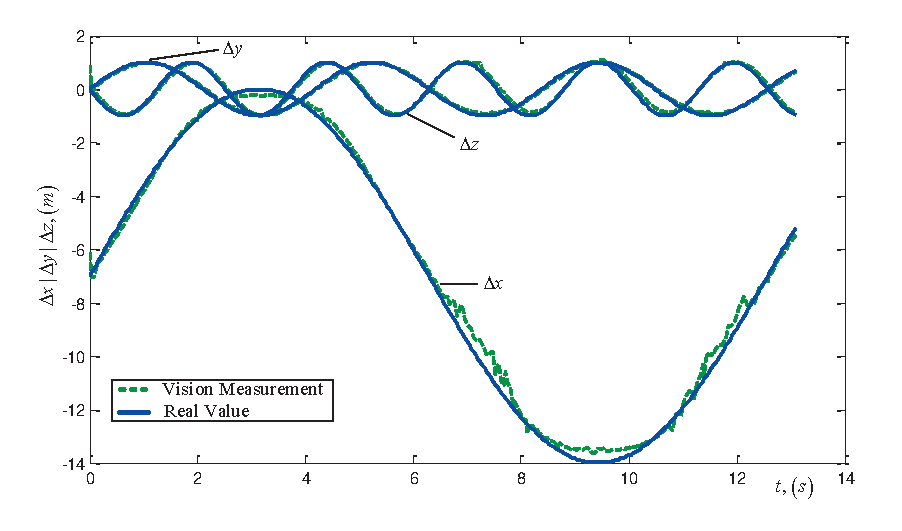
\includegraphics[width=0.7\hsize]{Figures/Figs_Ch6/duibi1.eps}
	\caption{The effect of visual location and tracking.}
	\label{fig8}
\end{figure}

In Fig.~\ref{fig8}, the dotted line represents the relative distance solved
by vision-based position estimation algorithm, while the solid line
represents the real distance. It can be obtained that the system can obtain fairly good localization information of
the drogue.

\section{Chapter Summary}

In this research, a vision-based position estimation method for
probe-and-drogue refueling systems is presented. These real-time detecting
and matching algorithms are of strong robustness. Through the simulation, the effectiveness and accuracy
of the proposed method have been demonstrated. Therefore, the proposed vision-based
position estimation method is promising to acquire the relative distance
information between the drogue and the receiver aircraft, which can be later
applied to the autonomous aerial refueling system.

In future research, the proposed method could be tested with a real camera, such as in a hardware-in-the-loop simulation. Besides, some other extreme
circumstances which may happen in real flight should be considered.